\section{Introduction}
\label{sec:ipsn-intro}

The RF spectrum is a natural resource in great demand due to the
unabated increase in mobile (and hence, wireless) data
consumption~\cite{Jeffrey14}.  The research community has
addressed this capacity crunch via development of {\em shared spectrum
  paradigms}, wherein the spectrum is made available to unlicensed
users (secondaries) as long as they do not interfere with the
transmission of licensed incumbents (primaries).  E.g., in the recent
years, the FCC has made available the CBRS band, i.e., the 3550-3700
MHz band within the 3.5 GHz band, for shared commercial use to allow
other users to utilize the otherwise low-usage band which was
previously reserved for incumbent users including US Navy radar
operators.


\begin{figure}[t]
\centering
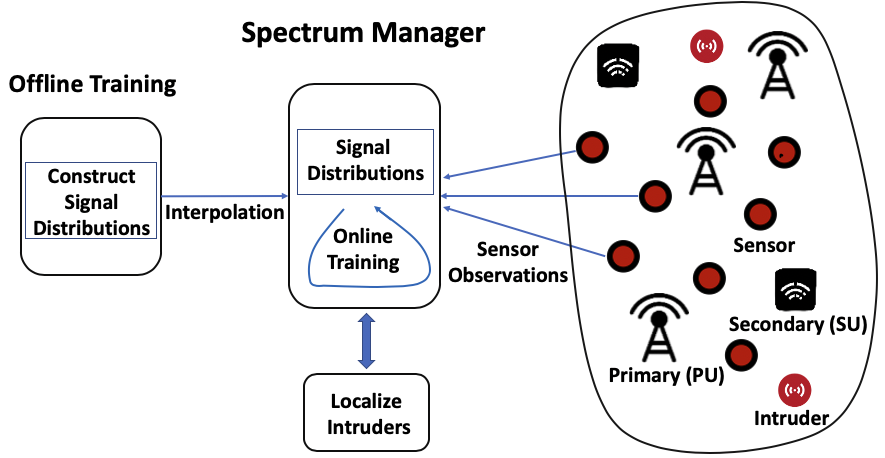
\includegraphics[width=0.95\textwidth]{chapters/ipsn/figures/architecture.png}
\caption{Overall approach to localize intruders in a shared spectrum system.} 
\label{fig:illustration}
\end{figure}

The increasing affordability of the software-defined radio (SDR)
technologies makes the shared spectrums particularly prone to
unauthorized usage or security attacks. With easy access to SDR
devices~\cite{usrp,hackrf}, it is easy for selfish users to transmit data
on shared spectrum without any authorization and potentially causing
harmful interference to the incumbent users.  Such illegal spectrum
usage could also happen as a result of infiltration of computer virus
or malware on SDR devices.  As the fundamental objective behind such
shared spectrum paradigms is to maximize spectrum utilization, the
viability of such systems depends on the ability to effectively guard
the shared spectrum against unauthorized usage.  The current
mechanisms however to locate such unauthorized users (intruders) are
human-intensive and time-consuming, involving FCC enforcement bureau
which detects violations via complaints and manual
investigation~\cite{mobicom17-splot}. 
\eat{As explained below, an effective
technique should be able to accurately localize multiple simultaneous
intruders and even in the presence of dynamically changing set of
authorized users.}
Motivated by above, we seek for an effective
technique that is able to accurately localize multiple simultaneous
intruders and even in the presence of dynamically changing set of
authorized users. In the following, we begin with describing the multiple transmitter localization problem.


%%% Multi-tx and challenges.
\para{Multiple-Transmitter Localization (MTL).}  \eat{Localization of
unauthorized users in a shared spectrum system essentially boils down to localizing transmitters/intruders in a given area under a shared spectrum system.}
 The transmitter localization problem has been well-studied, but most of the focus has been on localizing a {\em single} intruder at a time. However, it is important to localize multiple transmitters simultaneously to effectively guard a shared spectrum
system. E.g., a malware or virus-based attachment could simultaneously cause many devices to violate spectrum allocation rules; spectrum
jamming attacks would typically involve multiple transmitters. More
importantly, a technique limited by localization of a single intruder
could then be easily circumvented by an offender by using multiple
devices.
The key challenge in solving the MTL problem comes from the fact that
the deployed sensor would receive only a sum of the signals from multiple transmitters, and separating the signals may be impossible.  In
addition, the other challenge that MTL in the context of shared
spectrum system poses is the presence of authorized users---e.g., the
incumbent users and the dynamic set of secondary users that have been
allocated spectrum by the manager. To the best our knowledge, no prior
localization work has considered the presence of authorized users.

%%%% SPLOT and shortcomings.
The state-of-the-art technique for the MTL problem is the recent
work~\cite{mobicom17-splot}, which essentially decomposes the MTL
problem to multiple single-transmitter localization problems based on
the sensors with the highest power readings in a
neighborhood. \eat{To the best of our knowledge, this is the only
  work that has addressed the MTL problem extensively, especially in
  the context of shared spectrum systems.} However, the technique has
a few shortcomings: (i) it implicitly assumes a propagation model, and
thus, may not work effectively in areas with complex propagation
characteristics, (ii) it is not effective in the case of transmitters
being located close-by (a key challenging scenario for MTL problem),
and (iii) most importantly, it can't be extended effectively to
incorporate background authorized users, a key requirement in the
context of shared spectrum systems. 
\eat{In our evaluation, we
  have compared our technique with theirs and one other approach.}
%%\blue{Our localization approach belongs to the fingerprinting~\cite{infocom00-radar} category.}

%%%%%%%W WHAT we DO.
\para{Our Approach.}  Transmitter localization is generally done based
on observations at deployed sensors. In particular, as in prior
works~\cite{mobicom17-splot,chakraborty2017specsense}, we assume a
crowdsourced sensing architecture wherein relatively low-cost spectrum
sensors are available for gathering signal strength in the form of
received power. Our approach is a hypothesis-driven Bayesian approach,
viz.\ {\em maximum a posteriori} (\map) approach, wherein each
hypothesis is a configuration (i.e.  a combination of $\langle
location, power \rangle$ pair) of the potential intruders, and the
goal is to determine the hypothesis that best explains the sensor
observations. This determination is done based on the distributions
(gathered during a training phase) of sensor observations for each
hypothesis.
%%%%%%%%%%%%


%%%%% MOTIVATION.
\softpara{Motivation for \map.}  Our motivation for using a \map-based
approach is multifold: First, with sufficient training data, \map is
known to deliver optimal classification accuracy for the MTL problem.
Second, the \map approach doesn't assume any propagation model and
thus works for arbitrary signal propagation characteristics. Third, it
allows us to also estimate the intruder's transmit power, which can be
very useful in some applications, e.g., where the penalty is
proportional to the extent of violation. Lastly and most importantly,
it naturally extends to being able to handle a presence of an evolving
set of authorized users.

\softpara{Optimization and Novel Interpolation.} 
The benefits of a \mtl-based approach come at a cost. It
(i) incurs prohibitive computation cost---exponential in number of
potential intruders---when applied to the \mtl problem, and (ii)
requires significant amount of training cost. The focus of our work is
to address these challenges, and design a viable \map-based approach.

\emph{Optimization}. Using \map as a building block, we develop an optimized
approach that runs in polynomial time with minimized training cost using a divide-and-conquer idea.
We extend our technique to work in presence of authorized users by
incorporating online (real-time) training, which is enabled by utilizing some wireless signal charecteristics and thus incurs minimal cost.
\eat{We note that the online training to incorporate presence of authorized users is needed only for the prevailing setting (of authorized transmitters and deployed sensors) and hence incurs minimal cost
(see~\S\ref{sec:auth}). }

\blue{\emph{Novel Interpolation}. The \map framework requires prior
training to build probability distributions (PDs) of sensor
observations for each hypothesis.
In our work, we reduce the number of PDs to be constructed via a novel
interpolation scheme suited to our unique setting, and evaluate the
impact of reduced training on the localization accuracy.}

\para{Overall Contributions.}  The goal of our work is to develop an
efficient technique for accurate localization of simultaneously
present multiple intruders in a shared spectrum system. In this
context, we make the following specific contributions. 
\begin{enumerate}
\item
Design an efficient localization algorithm, i.e. \ouralgo, for the MTL problem, based
on an optimal hypotheses-driven Bayesian approach. The designed
approach predicts locations and transmit powers of the intruders, and
does not assume any propagation model and thus, works for arbitrary
signal propagation characteristics.

\item
Extend the designed algorithm to \ouralgoss, to localize effectively in the presence
of background authorized users, i.e., primaries with possibly unknown
parameters (e.g., location and transmit power) and an evolving set of
secondary users.

\item
Develop an effective interpolation scheme, i.e. \ildw, for our unique setting to
reduce the one-time training cost of our scheme, without impacting the
localization accuracy much.

\item
Evaluate our techniques via large-scale simulations as well as over
two developed testbeds (indoor and outdoor), and demonstrate the
effectiveness of our developed techniques and their superior
performance compared to the best-known techniques.
\end{enumerate}

%% We assume a crowdsourced architecture~\cite{}, wherein spectrum
%% sensing is delegated to independently deployed low-cost spectrum
%% sensors, such as rtl-sdr, who is merely over 20 dollars \cite{}.
%% Also there is a cloud-based spectrum manager~\cite{}, which 
%% orchestrates allocation of spectrum in such shared spectrum systems, 
%% based on available parameters and known channel conditions. 

%% The crowdsourcing spectrum sensor system scales well and realizes a
%% widespread and very cost-effective deployment.  Furthermore, it
%% facilitates the core spectrum management task we target at: guarding
%% the spectrum from unauthorized users.

%% Due to privacy, bandwith, and
%% cost concerns, it is impractical for the cheap sensors to send the
%% large raw signal I/Q samples to the cloud server.  Thus received
%% signal strength (RSS) is our choice of signal metrics.  So the sensors
%% process the raw signal I/Q samples locally and get RSS values, then
%% send the RSS values to the cloud.  Offloading the computation of
%% processing raw signal samples to the edge significantly decrease the
%% communication cost and enhance privacy.  T

% The best approach to date is \splot \cite{mobicom17-splot}, which utilized matrix inversion (essentially a variant of ridge regression) as a building block. However, it has an array of drawbacks. 
%% First and foremost, it is unable to localize two or more transmitters close by. 
%% The sensors' received signal is a phasor sum of the signals of both and \splot will report only one transmitter in the local maximum confined area.
%% Second, although it predicts location, it cannot predict the power of the transmitter. \splot is returning the coefficients of the ridge regression like function. 
%% The coefficients are correlated to the real power, but power is definitely not a function of those coefficients.
%% Third, the intrinsic mechanism of \splot assumes a propagation model.
%% They use a log normal model with an exponent of 2. However, the real environment may be more complicated than an ideal model, i.e. terrains can block and/or create multi-path reflection on the crowdsourced sensors.

%% The above three drawbacks comes from the settings of localizing only multiple illegal transmitters.
%% A fourth drawback will arise in the emerging shared spectrum system, where background transmissions from authorized users and potentially unauthorized offenders mixes together makes the proEvaluate our techniques via large-scale simulations as well as over
%two developed testbeds (indoor and outdoor), and demonstrate the
%effectiveness of our developed techniques and their superior
%performance compared to the best known techniques.blem harder by largely increasing the number of transmitters that need to be localized.
%% Multiple transmitter localization will hardly be perfect.
%% The more transmitters that need to localize, the less accuracy it gets.
%% For \splot, we see no good way of utilizing the information of authorized users to facilitate the localization of unauthorized offenders.
%% The way for \splot to work in a shared spectrum settings is to blindly localize all the transmitters and remove the known authorized users, then remains the unauthorized ones.
%% With this strategy, a smart spectrum offender can move close to an authorized user and safely transmit. 
%% \ble{In the mobicom-17 paper, they have a paragraph for dynamic localization, we might need to talk about it. It is a little related to our changing secondaries setting.}x
